% This example is meant to be compiled with lualatex or xelatex
% The theme itself also supports pdflatex
\PassOptionsToPackage{unicode}{hyperref}
\documentclass[aspectratio=1610, 9pt]{beamer}

% Warning, if another latex run is needed
% \usepackage[aux]{rerunfilecheck}

% just list chapters and sections in the toc, not subsections or smaller
\setcounter{tocdepth}{1}

%------------------------------------------------------------------------------
%------------------------------ Fonts, Unicode, Language ----------------------
%------------------------------------------------------------------------------
\usepackage{fontspec}
\defaultfontfeatures{Ligatures=TeX}  % -- becomes en-dash etc.

% german language
\usepackage{polyglossia}
\setdefaultlanguage{german}

% for english abstract and english titles in the toc
\setotherlanguages{english}

% intelligent quotation marks, language and nesting sensitive
\usepackage[autostyle]{csquotes}

% microtypographical features, makes the text look nicer on the small scale
\usepackage{microtype}

%------------------------------------------------------------------------------
%------------------------ Math Packages and settings --------------------------
%------------------------------------------------------------------------------

\usepackage{amsmath}
\usepackage{amssymb}
\usepackage{mathtools}
\usepackage{bbold}

% Enable Unicode-Math and follow the ISO-Standards for typesetting math
\usepackage[
  math-style=ISO,
  bold-style=ISO,
  sans-style=italic,
  nabla=upright,
  partial=upright,
]{unicode-math}
\setmathfont{Latin Modern Math}

% nice, small fracs for the text with \sfrac{}{}
\usepackage{xfrac}


%------------------------------------------------------------------------------
%---------------------------- Numbers and Units -------------------------------
%------------------------------------------------------------------------------

\usepackage[
  locale=DE,
  separate-uncertainty=true,
  per-mode=symbol-or-fraction,
]{siunitx}
\sisetup{math-micro=\text{µ},text-micro=µ}
% \sisetup{tophrase={{ to }}}
%------------------------------------------------------------------------------
%-------------------------------- tables  -------------------------------------
%------------------------------------------------------------------------------

\usepackage{booktabs}       % \toprule, \midrule, \bottomrule, etc

%------------------------------------------------------------------------------
%-------------------------------- graphics -------------------------------------
%------------------------------------------------------------------------------

\usepackage{graphicx}
%\usepackage{rotating}
\usepackage{grffile}
\usepackage{tikz}
\usepackage{circuitikz}
\usepackage{tikz-feynman}
\usepackage{subcaption}

% allow figures to be placed in the running text by default:
\usepackage{scrhack}
\usepackage{float}
\floatplacement{figure}{htbp}
\floatplacement{table}{htbp}

% keep figures and tables in the section
\usepackage[section, below]{placeins}


%------------------------------------------------------------------------------
%---------------------- customize list environments ---------------------------
%------------------------------------------------------------------------------

\usepackage{enumitem}
\usepackage{listings}
\usepackage{hepunits}

\usepackage{pdfpages}
%------------------------------------------------------------------------------
%------------------------------ Bibliographie ---------------------------------
%------------------------------------------------------------------------------

\usepackage[
  backend=biber,   % use modern biber backend
  autolang=hyphen, % load hyphenation rules for if language of bibentry is not
                   % german, has to be loaded with \setotherlanguages
                   % in the references.bib use langid={en} for english sources
]{biblatex}
\addbibresource{references.bib}  % the bib file to use
\DefineBibliographyStrings{german}{andothers = {{et\,al\adddot}}}  % replace u.a. with et al.


% Load packages you need here
% \usepackage{polyglossia}
% \setmainlanguage{german}

\usepackage{csquotes}


% \usepackage{amsmath}
% \usepackage{amssymb}
% \usepackage{mathtools}

\usepackage{hyperref}
\usepackage{bookmark}

% load the theme after all packages

\usetheme[
  showtotalframes, % show total number of frames in the footline
]{tudo}

% Put settings here, like
\unimathsetup{
  math-style=ISO,
  bold-style=ISO,
  nabla=upright,
  partial=upright,
  mathrm=sym,
}

% \setbeamertemplate{itemize item}{\scriptsize$\blacktriangleright$}
% \setbeamertemplate{itemize subitem}{\scriptsize$\blacktriangleright$}

%Titel:
\title{Gamma-Spectroscopy}
%Autor
\author[N.Breer]{Nils Breer}
%Lehrstuhl/Fakultät
\institute{Fakultät Physik}
%Titelgrafik muss ich einfueren!!!
%\titlegraphic{\includegraphics[width=0.3\textwidth]{content/Bilder/interferenz.jpg}}
\date{12.07.2022}

\begin{document}
\maketitle

\begin{frame}\frametitle{Agenda}
  \begin{itemize}
    \item What is gamma spectroscopy?
    \item Interactions in the Spectrum
    \item Detectorsystems
    \item Applications
    \item Summary
  \end{itemize}
\end{frame}

\begin{frame}\frametitle{What is gamma spectroscopy?}
  \begin{itemize}
    \item studies of energy spectra of gamma rays
    \item identification of gamma emitting radionuclides
    % \item TL:DR : photons enter matter and interact with free or bound electrons, nuclides or fields
    % \item interaction processes: $E_\gamma$, Z from absorber
  \end{itemize}
\end{frame}

\begin{frame}\frametitle{Interactions}
  \begin{itemize}
    \item Photoeffect
    \item Comptoneffect
    \item Pair production
  \end{itemize}
\end{frame}

\begin{frame}\frametitle{Photoeffect}
  \begin{itemize}
    \item photon interacts with huellen electrons
    \item $\gamma + atom \to atom^{+} + e^{-}$
    \item hole is filled with electrons from higher orbitals recursively
    \item energy difference are characteristic and photons are released as x-rays
    \item rarely: photon leaves absorber. often excite more electrons inside
    \item K-L-M-absorption edge: Quantumenergy enough to release bound electron from given state
  \end{itemize}
\end{frame}

\begin{frame}\frametitle{Compton scattering}
  \begin{columns}
    \begin{column}[c]{0.48\textwidth}
      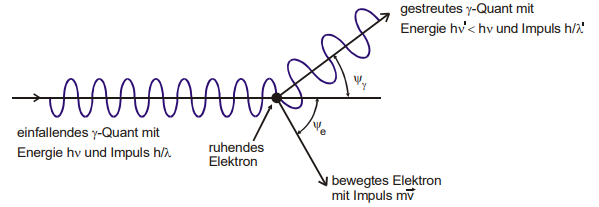
\includegraphics[width=\textwidth]{plots/compton.png}
    \end{column}
    \begin{column}[c]{0.48\textwidth}
      \begin{itemize}
        \item inelastic scattering
        \item photons only transfers a fraction of its energy
        \item bad! cannot view full spectrum
      \end{itemize}
    \end{column}
  \end{columns}
\end{frame}

\begin{frame}\frametitle{Compton scattering}
  \begin{columns}
    \begin{column}[c]{0.48\textwidth}
      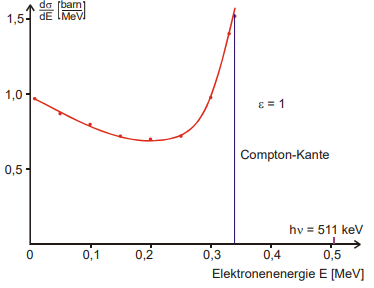
\includegraphics[width=\textwidth]{plots/compton_kante.png}
    \end{column}
    \begin{column}[c]{0.48\textwidth}
      \begin{itemize}
        \item non-isotropic angular distribution
        \item keV: thomson'sche scatter cross section: $\sigma_{th} = \frac{8}{3}\pi r_e^2$
        \item $\frac{\symup{d}\sigma}{\symup{d}E} = \frac{3}{8}\sigma_{th}\frac{1}{m_0 c^2 \epsilon^2}
        (2 + (\frac{E}{h\nu - E})^2(\frac{1}{\epsilon^2} + \frac{h\nu - E}{h\nu}-\frac{2}{\epsilon}(\frac{h\nu - E}{h\nu})))$
      \end{itemize}
    \end{column}
  \end{columns}
\end{frame}

\begin{frame}\frametitle{Pair production}
  \begin{columns}
    \begin{column}[c]{0.48\textwidth}
      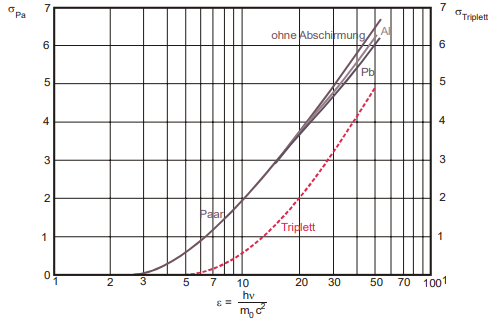
\includegraphics[width=\textwidth]{plots/pair_triplett.png}
    \end{column}
    \begin{column}[c]{0.48\textwidth}
      \begin{itemize}
        \item photon produces e+e- pair if E is high enough
        \item can only occur in proximity of nucleus/scattering partner
        \item in restframe photon mass = 0, lepton mass > 0; someone needs to take the momentum
        \item photon line visible if both leptons are absorbed; different lines if leptons escape (BREMSSTRAHLUNG)
        \item annihilation peak : 511 keV (e- mass) or doubled for both
      \end{itemize}
    \end{column}
  \end{columns}
\end{frame}

\begin{frame}\frametitle{Germanium detector}
  \begin{columns}
    \begin{column}[c]{0.48\textwidth}
      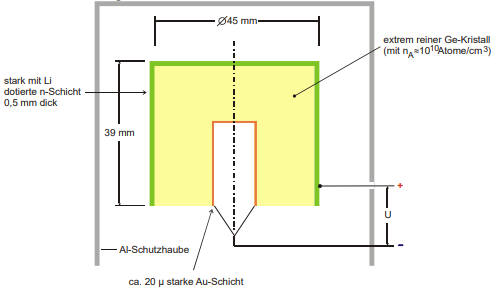
\includegraphics[width=\textwidth]{plots/ge.png}
    \end{column}
    \begin{column}[c]{0.48\textwidth}
      % \textbf{c}
      \begin{itemize}
        \item germanium semiconductor
        \item solid detection material for full energy deposition inside
        \item gas: only partial deposition
        \item electrical properties needed for electron-hole pairs to electric signal!
        \item also possible: scintillators -> trap photons and use SiPMs
      \end{itemize}
    \end{column}
  \end{columns}
\end{frame}

\begin{frame}{Band structure}
  \begin{itemize}
    \item electrons in discrete/precise energy bands with fixed number of e-
    \item valence band: outer band for chemical reactions; most inhibited
    \item electrons must move between bands to migrate the material
  \end{itemize}
\end{frame}

\begin{frame}{Semi conductor}
  \begin{itemize}
    \item small band gap between valence band and conduction band (1 eV)
    \item few e- in conduction band -> limited conductivity
    \item migration proportional to Temparture T
    \item $p(T) = T^{3/2} \times exp(-E_g / 2 k_b T)$
  \end{itemize}
\end{frame}

\begin{frame}\frametitle{How to semiconductor}
  \begin{itemize}
    \item p and n doped areas
    \item charge carriers diffuse and recombinate
    \item surface is charge carrier poor zone
    \item  acceptor in p, donator in n _. electric field hinders carriers
    \item the bigger the zone the better the seperation -> more $U_g$
    \item seperation before recombination -> pulse -> quatification of energy
    \item only possible if generated in depletion zone (charge carrier poor zone)
    \item depletion zone big -> reverse voltage and doping material
    \item asymmetric doping (equation)
    \item noise: electrons randomly passing reverse voltage, also cool detector
    \item veto region with alu case ($E_{min} = 40 - 50 keV$)
    \item Li in Ge for n, Au in Ge for p
  \end{itemize}
\end{frame}

\begin{frame}\frametitle{why is gamma spectroscopy better than radio chemistry?}
  \begin{columns}
    \begin{column}[c]{0.48\textwidth}
      PRO:
      \begin{itemize}
        \item less expensive
        \item fast
        \item multinuclide analysis (distinct lines visible for all nuclides)
        \item non-destructive for emitter (radiation hardness of detector given)
        \item remote measurement
      \end{itemize}
    \end{column}
    \begin{column}[c]{0.48\textwidth}
      CONTRA:
      \begin{itemize}
        \item often less sensitive
        \item require large sample masses (if not gamma rays from space)
      \end{itemize}
    \end{column}
\end{frame}

\begin{frame}\frametitle{Table of interesting radio nuclides}
  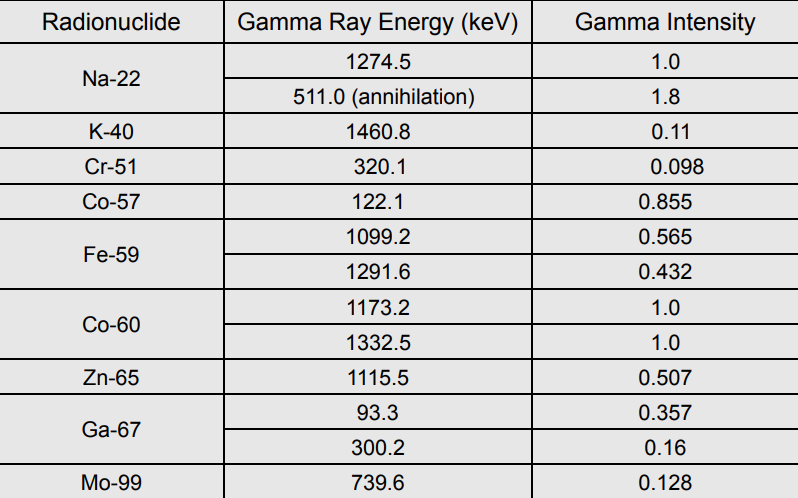
\includegraphics[width=\textwidth]{plots/nuclid_table1.png}
\end{frame}

\begin{frame}\frametitle{Summary}
  \begin{itemize}
    \item f
  \end{itemize}
\end{frame}

\begin{frame}\frametitle{Quellen}
% \url{http://www.telescopearray.org/index.php/about/telescope-array} \\
% \url{https://www.researchgate.net/figure/A-schematic-of-the-Pierre-Auger-Observatory-where-each-black-dot-is-a-water-Cherenkov_fig1_319524774} \\
% \url{https://www.cta-observatory.org/pevatrons-hunt-for-galactic-cosmic-rays/} \\
% \url{https://arxiv.org/pdf/2105.06148.pdf} \\
% \url{https://doi.org/10.1007/978-3-319-63411-1_1} \\
% \url{https://www.sciencedirect.com/science/article/pii/S0927650512000382} \\
% \url{https://cerncourier.com/a/lhcbs-momentous-metamorphosis/} \\
% \url{https://arxiv.org/pdf/1412.5106.pdf} \\
% \url{https://www.epj-conferences.org/articles/epjconf/pdf/2019/14/epjconf_ricap2019_01015.pdf} \\
% \url{https://pos.sissa.it/358/890/pdf} \\
\end{frame}

\end{document}

% \begin{frame}\frametitle{}
%   \begin{columns}
%   \begin{column}[c]{0.45\textwidth}
%     \begin{itemize}
%       \item
%       \item
%       \item
%       \item
%     \end{itemize}
%   \end{column}
%   \begin{column}[c]{0.45\textwidth}
%     % \includegraphics{images/icecube.png}
%   \end{column}
%   \end{columns}
% \end{frame}
